\documentclass[aspectratio=169,11pt]{beamer}
\usetheme{Madrid}
\usecolortheme{default}
\usepackage[T1]{fontenc}
\usepackage{lmodern}
\usepackage{tikz}
\usetikzlibrary{positioning}
\usepackage{xcolor}
\usepackage{booktabs,tabularx,amsmath,listings,tikz,graphicx}
\usetikzlibrary{arrows.meta,positioning}
\definecolor{navy}{HTML}{142B4A}\definecolor{blue}{HTML}{2463A6}\definecolor{pale}{HTML}{EEF4FA}\definecolor{green}{HTML}{247A58}
\setbeamercolor{structure}{fg=blue}\setbeamercolor{frametitle}{bg=navy,fg=white}\setbeamercolor{title}{fg=white}\setbeamercolor{block title}{bg=blue,fg=white}\setbeamercolor{block body}{bg=pale,fg=black}
\setbeamertemplate{navigation symbols}{}
% Clean presentation chrome: no repeated author/title header or team-name footer.
\setbeamertemplate{headline}{}
\setbeamertemplate{footline}{%
  \leavevmode%
  \hbox{%
    \begin{beamercolorbox}[wd=\paperwidth,ht=2.6ex,dp=1.1ex,rightskip=1em]{author in head/foot}%
      \hfill\color{navy}\insertframenumber/\inserttotalframenumber
    \end{beamercolorbox}%
  }%
}

\lstset{basicstyle=\ttfamily\scriptsize,backgroundcolor=\color{pale},frame=single,breaklines=true,showstringspaces=false}
\title[Algorithm Benchmarking Suite]{Algorithm Benchmarking and Profiling Suite}
\subtitle{Software Systems Lab Project \;|\; CS202C}
\institute{\large Indian Institute of Technology Dharwad\\Faculty: Dr. Suman Dutta}
\date{November 2026}
\begin{document}
\begin{frame}[plain]
\titlepage
\vspace{-0.4cm}
\centering \underline{Project Team}
\begin{center}
\small
Abhinav -- CS25BT028 \quad Jyoteen -- CS25BT064\\
Shyam -- CS25BT061 \quad Gaurav -- CS25BT024\\
Harsh -- CS25BT019
\end{center}
\end{frame}
\begin{frame}{Why benchmark algorithms?}
\begin{itemize}
\item Big-O analysis explains how an algorithm scales as input grows.
\item Real execution time is also affected by constant factors, memory behaviour, compiler settings and the machine.
\item A benchmark provides measured evidence; a profiler helps investigate where execution time is spent.
\end{itemize}
\begin{block}{Project goal}
Build a repeatable workflow that compares two selected sorting algorithms on the same generated datasets, measures their CPU time, profiles them separately and plots the results.
\end{block}
\end{frame}
\begin{frame}{Project objectives and scope}
\begin{enumerate}
\item Select two distinct sorting implementations through a command-line interface.
\item Generate reproducible integer datasets for multiple input sizes.
\item Compile both algorithms using a shared runner and common flags.
\item Measure repeated runs and summarize with the median.
\item Generate separate profiler reports and a runtime comparison graph.
\end{enumerate}
\vspace{0.3cm}
\textbf{Scope note:} The current interactive workflow benchmarks two sorting algorithms per execution. Search and summation source files are present in the repository but are not part of this workflow.
\end{frame}
\begin{frame}{Algorithms available}
\begin{columns}[T]
\column{0.5\textwidth}
\begin{block}{Elementary comparison sorts}
\begin{itemize}
\item Bubble sort
\item Cocktail Shaker sort
\item Gnome sort
\item Insertion sort
\item Odd--Even Transposition sort
\item Selection sort
\end{itemize}
\end{block}
\column{0.5\textwidth}
\begin{block}{Alternative sorting strategies}
\begin{itemize}
\item Heap sort — $O(n\log n)$
\item Merge sort — $O(n\log n)$
\item Tuned merge sort — profiling-guided variant
\item Quicksort — average $O(n\log n)$
\item Radix sort — four byte passes
\item Shell sort — Ciura gap sequence
\end{itemize}
\end{block}
\end{columns}
\small The source filenames label some routines as ``unoptimized'' or ``optimized''; this is a project naming convention, not a guaranteed performance ranking.
\end{frame}
\begin{frame}{System architecture}
\centering
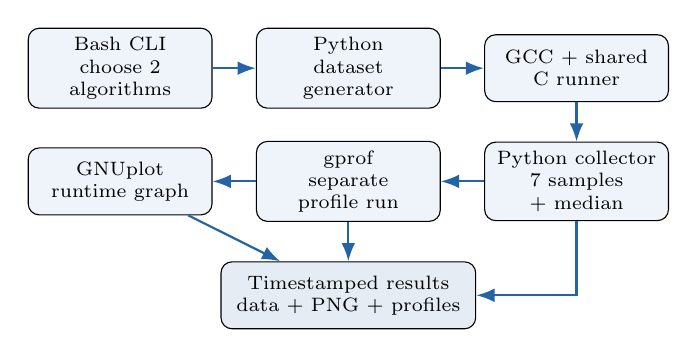
\begin{tikzpicture}[node distance=0.5cm and 0.55cm,every node/.style={draw,rounded corners,align=center,minimum height=0.85cm,text width=2.1cm,font=\scriptsize},arr/.style={-{Latex},thick,draw=blue}]
\node[fill=pale] (cli) {Bash CLI\\choose 2 algorithms};
\node[fill=pale,right=of cli] (gen) {Python\\dataset generator};
\node[fill=pale,right=of gen] (gcc) {GCC + shared\\C runner};
\node[fill=pale,below=of gcc] (collect) {Python collector\\7 samples + median};
\node[fill=pale,left=of collect] (prof) {gprof\\separate profile run};
\node[fill=pale,left=of prof] (plot) {GNUplot\\runtime graph};
\node[fill=blue!12,below=of prof,text width=3cm] (result) {Timestamped results\\data + PNG + profiles};
\draw[arr](cli)--(gen);\draw[arr](gen)--(gcc);\draw[arr](gcc)--(collect);\draw[arr](collect)--(prof);\draw[arr](prof)--(plot);\draw[arr](collect)|-(result);\draw[arr](prof)--(result);\draw[arr](plot)--(result);
\end{tikzpicture}
\vspace{0.25cm}
\small The Bash script coordinates the complete pipeline and checks that required tools and output files are available.
\end{frame}
\begin{frame}{Dataset generation}
\begin{itemize}
\item Input sizes: $100,150,200,\ldots,1000$ — 19 datasets.
\item For each size $n$, seed = $2026+n$.
\item Generate $n$ integers uniformly through Python's \texttt{randrange(0, 1000000)}.
\item Values lie in $[0,999999]$; this also satisfies the radix-sort implementation's non-negative-key assumption.
\item Both selected algorithms receive the same saved dataset for each input size.
\end{itemize}
\begin{block}{Why use a fixed seed?}
It makes the input data reproducible, so a later run can use the same dataset sequence rather than comparing algorithms on unrelated random inputs.
\end{block}
\end{frame}

\begin{frame}[fragile]{Common C Interface and Benchmark Outputs}
Every sorting source implements the same function:

\begin{lstlisting}[language=C]
void algorithm(const int *input, int *output, int n);
\end{lstlisting}

\vspace{0.3cm}

\textbf{Outputs Produced by a Run}

\begin{tabularx}{\textwidth}{lX}
\toprule
\textbf{Output} & \textbf{What it contains}\\
\midrule
\texttt{datasets/} & The 19 generated input files.\\
\texttt{benchmark\_data.dat} & Input size and median seconds per sort for both algorithms.\\
\texttt{runtime\_comparison.png} & GNUplot line graph; logarithmic y-axis.\\
\texttt{profiles/} & Separate gprof reports for the selected algorithms.\\
\texttt{bin/} & Normal and profiling binaries and object files.\\
\bottomrule
\end{tabularx}

\vspace{0.3cm}

All outputs are saved in a unique timestamped directory under
\texttt{results/}.

\end{frame}

\begin{frame}{Benchmark results: Bubble Sort vs.\ Merge Sort}
\begin{columns}[T]
\column{0.64\textwidth}
\includegraphics[width=\linewidth,height=0.60\textheight,keepaspectratio]{runtime_comparison.png}

\column{0.36\textwidth}
\textbf{Measured values}
\begin{tabular}{r|r}
\textbf{$n$} & \textbf{Bubble / Merge}\\\hline
100 & 3.47$\times$\\
500 & 14.17$\times$\\
1000 & 17.01$\times$
\end{tabular}
\vspace{0.25cm}
\begin{block}{Observation}
At $n=1000$, Merge Sort was about 17.0 times faster in this reference run.
\end{block}
\end{columns}
\end{frame}
\begin{frame}{Profiling case study: tuning Merge Sort}
\begin{itemize}
\item gprof: \texttt{merge} = 95.4\% of time, 999 calls per sort
\item Fix 1: insertion sort for blocks of 16 or fewer elements
\item Fix 2: alternating buffers, no copy-back loop
\end{itemize}
\begin{center}
\begin{tabular}{|r|r|r|r|}
\hline
$n$ & Original (s) & Tuned (s) & Speedup\\
\hline
100 & $1.04\times10^{-5}$ & $4.51\times10^{-6}$ & 2.30$\times$\\
500 & $8.98\times10^{-5}$ & $3.32\times10^{-5}$ & 2.70$\times$\\
1000 & $2.23\times10^{-4}$ & $1.21\times10^{-4}$ & 1.85$\times$\\
\hline
\end{tabular}
\end{center}
\small \texttt{merge} calls per sort: 999 $\rightarrow$ 63. Measured on the team's machine.
\end{frame}
\begin{frame}[fragile]{How to execute the project}
From the project root on Linux or WSL:
\begin{lstlisting}[language=bash]
sudo apt update
sudo apt install build-essential binutils gnuplot \
  python3 python3-numpy
chmod +x main/run.sh tests/test.sh
bash tests/test.sh
./main/run.sh
\end{lstlisting}
Choose two different algorithm numbers when prompted. Or pass two source paths directly:
\begin{lstlisting}[language=bash]
./main/run.sh algorithms/dataset/bubble_unoptimized.c \
  algorithms/dataset/merge_optimized.c
\end{lstlisting}
\end{frame}


% =================================================
% TEAM MEMBERS AND ROLES
% =================================================

\begin{frame}{Team Member's Roles}

\begin{columns}[T,onlytextwidth]

% ABHINAV
\begin{column}{0.19\textwidth}
\begin{beamercolorbox}[
  wd=\linewidth,
  ht=4.65cm,
  dp=0cm,
  center,
  sep=0.08cm
]{block body}
\vbox to 4.45cm{
\centering
\vspace{0.05cm}


\begin{tikzpicture}
\node[circle,fill=blue!75!black,
minimum size=0.85cm,text=white,
font=\large\bfseries] {A};
\end{tikzpicture}

\vspace{0.15cm}
{\bfseries Abhinav}

\vspace{0.08cm}
{\scriptsize CS25BT028}

\vspace{0.25cm}
\parbox[t][1.65cm][t]{\linewidth}{
\centering\scriptsize
Bash automation, Dataset generation,
GNUplot, Folder Structure
}
\vfill
}
\end{beamercolorbox}
\end{column}


% JYOTEEN
\begin{column}{0.19\textwidth}
\begin{beamercolorbox}[
  wd=\linewidth,
  ht=4.65cm,
  dp=0cm,
  center,
  sep=0.08cm
]{block body}
\vbox to 4.45cm{
\centering
\vspace{0.05cm}


\begin{tikzpicture}
\node[circle,fill=teal!85!black,
minimum size=0.85cm,text=white,
font=\large\bfseries] {J};
\end{tikzpicture}

\vspace{0.15cm}
{\bfseries Jyoteen}

\vspace{0.08cm}
{\scriptsize CS25BT064}

\vspace{0.25cm}
\parbox[t][1.65cm][t]{\linewidth}{
\centering\scriptsize
Benchmarking both programs across dataset sizes}
\vfill
}
\end{beamercolorbox}
\end{column}


% SHYAM
\begin{column}{0.19\textwidth}
\begin{beamercolorbox}[
  wd=\linewidth,
  ht=4.65cm,
  dp=0cm,
  center,
  sep=0.08cm
]{block body}
\vbox to 4.45cm{
\centering
\vspace{0.05cm}


\begin{tikzpicture}
\node[circle,fill=orange!90!yellow,
minimum size=0.85cm,text=white,
font=\large\bfseries] {S};
\end{tikzpicture}

\vspace{0.15cm}
{\bfseries Shyam}

\vspace{0.08cm}
{\scriptsize CS25BT061}

\vspace{0.25cm}
\parbox[t][1.65cm][t]{\linewidth}{
\centering\scriptsize
README.md and
\texttt{requirements.txt}
}
\vfill
}
\end{beamercolorbox}
\end{column}


% GAURAV
\begin{column}{0.19\textwidth}
\begin{beamercolorbox}[
  wd=\linewidth,
  ht=4.65cm,
  dp=0cm,
  center,
  sep=0.08cm
]{block body}
\vbox to 4.45cm{
\centering
\vspace{0.05cm}


\begin{tikzpicture}
\node[circle,fill=red!75,
minimum size=0.85cm,text=white,
font=\large\bfseries] {G};
\end{tikzpicture}

\vspace{0.15cm}
{\bfseries Gaurav}

\vspace{0.08cm}
{\scriptsize CS25BT024}

\vspace{0.25cm}
\parbox[t][1.65cm][t]{\linewidth}{
\centering\scriptsize
LaTeX report, Beamer presentation,
Folder Structure
}
\vfill
}
\end{beamercolorbox}
\end{column}


% HARSH
\begin{column}{0.19\textwidth}
\begin{beamercolorbox}[
  wd=\linewidth,
  ht=4.65cm,
  dp=0cm,
  center,
  sep=0.08cm
]{block body}
\vbox to 4.45cm{
\centering
\vspace{0.05cm}


\begin{tikzpicture}
\node[circle,fill=gray!75!navy,
minimum size=0.85cm,text=white,
font=\large\bfseries] {H};
\end{tikzpicture}

\vspace{0.15cm}
{\bfseries Harsh}

\vspace{0.08cm}
{\scriptsize CS25BT019}

\vspace{0.25cm}
\parbox[t][1.65cm][t]{\linewidth}{
\centering\scriptsize
Test cases, Results,
Profiling tools, Documentation
}
\vfill
}
\end{beamercolorbox}
\end{column}

\end{columns}

\end{frame}


\begin{frame}{Conclusion}
\begin{block}{Conclusion}
The project integrates deterministic dataset generation, a reusable C runner, median-based timing, separate gprof profiling and GNUplot visualization into one repeatable pairwise sorting benchmark workflow.
\end{block}
\centering\vspace{1cm}
{\Huge\color{navy}\bfseries \underline {Thank You}}\par\vspace{0.5cm}
{\Large Questions?}\par\vspace{0.5cm}
\textbf{Software Systems Lab (CS202C)}\par
Indian Institute of Technology Dharwad\\Faculty: Dr. Suman Dutta
\end{frame}
\end{document}